\documentclass[pdf,xcolor={dvipsnames}]{beamer}
\usepackage{xcolor,soul}

\makeatletter
\newcommand\SoulColor{%
	\let\set@color\beamerorig@set@color
	\let\reset@color\beamerorig@reset@color}
\newcommand\titlecolor{\usebeamercolor[fg]{frametitle}}
\newcommand\red{\color{red}}
\makeatother

\mode<presentation>{\usetheme{default}}
\title{An Efficient Exact Solution to the \newline ($l$,$d$) Planted Motif Problem}
\author{Maria Clara Isabel Sia*\\Julieta Nabos\\Proceso Fernandez}

\begin{document}
\begin{frame}\titlepage\end{frame}

\begin{frame}{Introduction}{The ($l,d$) planted motif problem}	
	\only<1>{\centering
		\emph{Find a motif of length {\titlecolor $l$=8} across these DNA sequences.}\\
		\emph{Each contains the motif with at most {\titlecolor $d$=2} mismatches.}\\\ \\
		\small
		$\titlecolor S_1$\ \ \  
		\texttt{atcactcgttctcctctaatgtgtaaagacgtactaccgacctta}
		\ \ \ \ \ \ \\\ \\

		$\titlecolor S_2$\ \ \  
		\texttt{acgccgaccggtccgatccttgtatagctcctaacgggcatcagc}
		\ \ \ \ \ \ \\\ \\

		$\titlecolor S_3$\ \ \  
		\texttt{tcctgactgcatcgcgatctcggtagtttcctgttcatcattttt}
		\ \ \ \ \ \ \\\ \\

		$\titlecolor S_4$\ \ \  
		\texttt{ggccctcagcatcgtgcgtcctgctaacacattcccatgcagctt}
		\ \ \ \ \ \ \\\ \\
		
		$\titlecolor S_5$\ \ \  
		\texttt{tgaaaagaatttacggtaaaggatccacatccaatcgtgtgaaag}
		\ \ \ \ \ \ \\\ \\\ \\

		\emph{Planted motif: }\texttt{\ \ \ ?\ ?\ \ \ \ }\\
		}

	\only<2>{\centering
		\emph{Find a motif of length {\titlecolor $l$=8} across these DNA sequences.}\\
		\emph{Each contains the motif with at most {\titlecolor $d$=2} mismatches.}\\\ \\
		\small
		$\titlecolor S_1$\ \ \  
		\texttt{at\SoulColor\hl{c{\color{red}a}{\color{red}c}tcgtt}ctcctctaatgtgtaaagacgtactaccgacctta}
		\ \ \ \ \ \ \\\ \\

		$\titlecolor S_2$\ \ \  
		\texttt{acgccgaccggtc\SoulColor\hl{c{\color{red}g}atc{\color{red}c}tt}gtatagctcctaacgggcatcagc}
		\ \ \ \ \ \ \\\ \\

		$\titlecolor S_3$\ \ \  
		\texttt{tcctgactgcatcgcgatctcggtagtttcctgt\SoulColor\hl{{\color{red}t}catc{\color{red}a}tt}ttt}
		\ \ \ \ \ \ \\\ \\

		$\titlecolor S_4$\ \ \  
		\texttt{ggccctca\SoulColor\hl{{\color{red}g}catcgt{\color{red}g}}\color{black}cgtcctgctaacacattcccatgcagctt}
		\ \ \ \ \ \ \\\ \\\color{black}
		
		$\titlecolor S_5$\ \ \  
		\texttt{tgaaaagaatttacggtaaaggatccacatc\SoulColor\hl{c{\color{red}a}atcgt{\color{red}g}}\color{black}tgaaag}
		\ \ \ \ \ \ \\\ \\\ \\

		\color{black}\emph{Planted motif: }\texttt{\SoulColor\hl{ccatcgtt}}\\
		}
	
	\only<3>{
		\begin{itemize}
		\item {\titlecolor motifs}: significant sub-sequences occuring repeatedly in DNA \\\ \\
		\item {\titlecolor DNA motif finding} must allow for mismatches due to mutation\\\ \\
		\item motif search is known as a difficult ({\titlecolor NP-complete}) problem in
		computational biology and CS \\\ \\
		\end{itemize}
		}

	\end{frame}

\begin{frame}{Introduction}{Key concepts}
	\only<1>{
	\begin{itemize}
		\setbeamercovered{transparent=25}
		\item {\titlecolor $l$-mer}
			\\- sequence of length $l$\\
			\begin{center}
			{\small $S_1$\ =\ \texttt{at{\color{red}c{ac}tcgtt}ctcctctaatgtgtaaagacgtactaccgacctta}\\ \ \\}
			\end{center}
		\item {\titlecolor Hamming distance $d_H$}
			\\- number of mismatches between $l$-mers\\
				\begin{columns}
					\begin{column}{0.1\textwidth}\end{column}
					\begin{column}{0.4\textwidth}
					\begin{center} {
						$x_1$ = \texttt{c{\color{red}g}atc{\color{red}c}tt}\ \ \\
						$x_2$ = \texttt{c{\color{red}c}atc{\color{red} g}tt}\ \ \\
					}\end{center}
					\end{column}
					\begin{column}{0.5\textwidth}
					% \begin{center} {
						$d_H(x_1,x_2) = 2$\ \ \\
					% }\end{center}
					\end{column}
				\end{columns}
			% \ \\ \vspace*{4pt} - $x_1$ and $x_2$ are considered {\titlecolor $d$-neighbors} if $d \geq 2$
		\end{itemize}}


	\only<2>{
	\begin{itemize}
	\item {\titlecolor $d$-neighborhood}\\
		- ex. the set of all {\red $d$-neighbors} of \texttt{acgt}, $d$=2:\\\ \\
		\texttt{\centering\small\ acgt, \\\vspace*{4pt}
			\ {\red c}cgt, {\red g}cgt, {\red t}cgt, a{\red a}gt, a{\red g}gt, a{\red t}gt,\\
			\ ac{\red a}t, ac{\red g}t, ac{\red t}t, acg{\red a}, acg{\red c}, acg{\red g},\\\vspace*{6pt}
			\ {\red ca}gt, {\red cg}gt, {\red ct}gt, {\red c}c{\red a}t, {\red c}c{\red c}t, {\red c}c{\red t}t, 
			  {\red c}cg{\red a}, {\red c}cg{\red c}, {\red c}cg{\red g},\\
			\ {\red ga}gt, {\red gg}gt, {\red gt}gt, {\red g}c{\red a}t, {\red g}c{\red c}t, {\red g}c{\red t}t, 
			  {\red g}cg{\red a}, {\red g}cg{\red c}, {\red g}cg{\red g},\\
			\ {\red ta}gt, {\red tg}gt, {\red tt}gt, {\red t}c{\red a}t, {\red t}c{\red c}t, {\red t}c{\red t}t, 
			  {\red t}cg{\red a}, {\red t}cg{\red c}, {\red t}cg{\red g},\\
			\ a{\red aa}t, a{\red ac}t, a{\red at}t, a{\red a}g{\red a}, a{\red a}g{\red c}, a{\red a}g{\red g}, 
			  a{\red ga}t, a{\red gc}t, a{\red gt}t,\\
			\ a{\red g}g{\red a}, a{\red g}g{\red c}, a{\red g}g{\red g}, a{\red ta}t, a{\red tc}t, a{\red tt}t, 
			  a{\red t}g{\red a}, a{\red t}g{\red c}, a{\red t}g{\red g},\\
			\ ac{\red aa}, ac{\red ac}, ac{\red ag}, ac{\red ca}, ac{\red cc}, ac{\red cg}, ac{\red ta}, ac{\red tc},
			  ac{\red tg}
		}\ \\\ \\
		\end{itemize}
		}
	\end{frame}

\begin{frame}{Problem statement}

	\end{frame}

\begin{frame}{EMS-GT}{Demonstration}
	\only<1>{\centering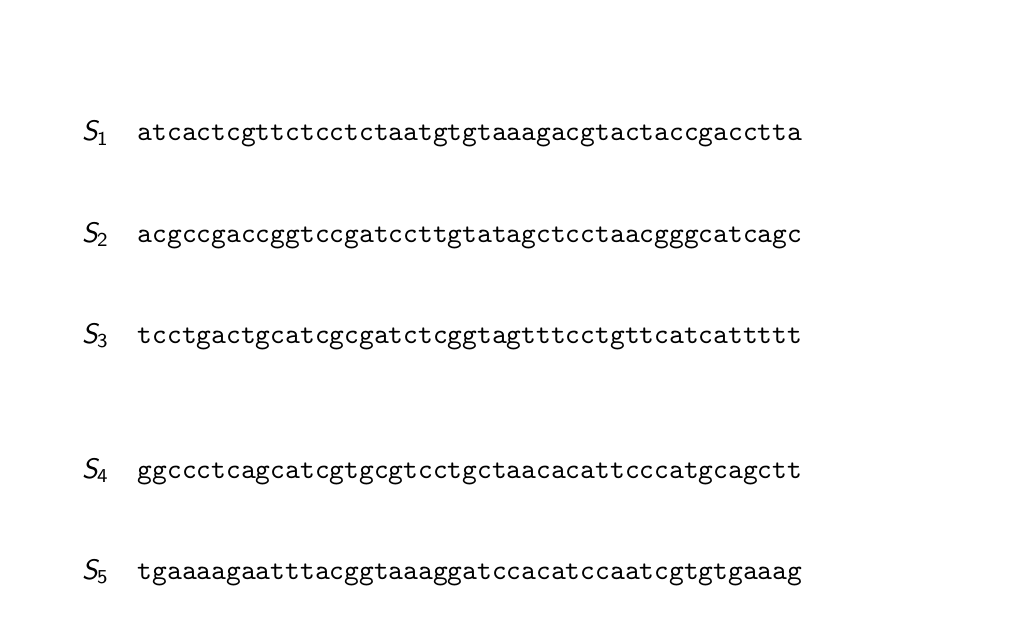
\includegraphics[width=\textwidth]{img/demo0}}
	\only<2>{\centering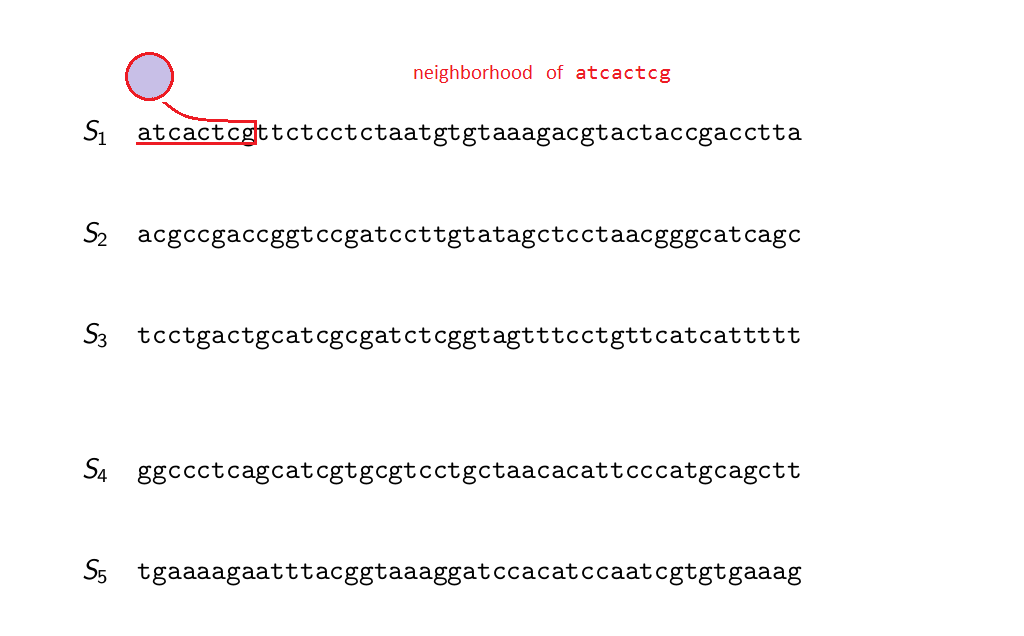
\includegraphics[width=\textwidth]{img/demo1}}
	\only<3>{\centering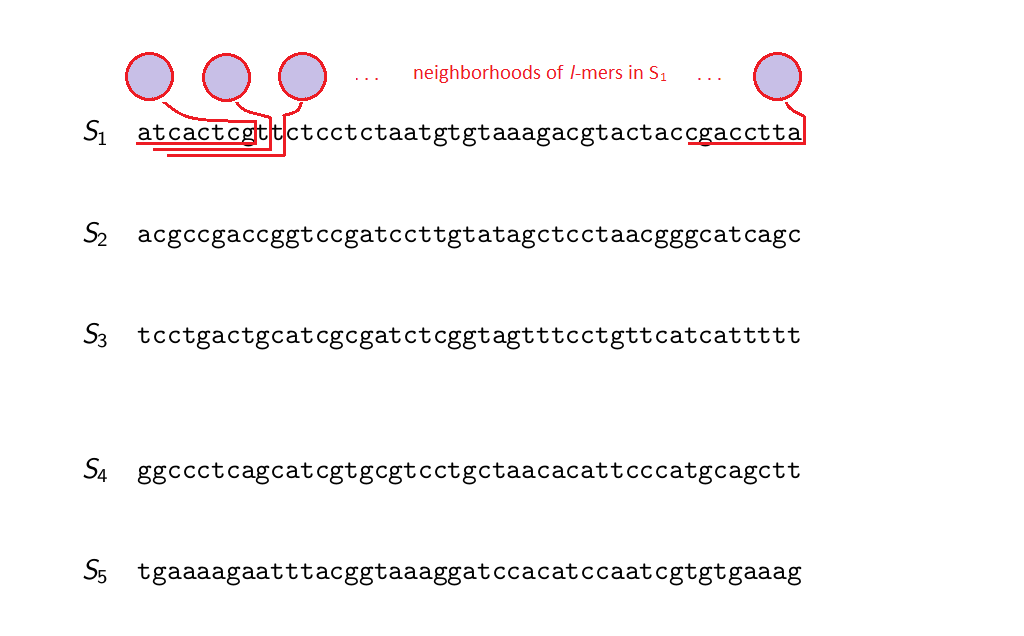
\includegraphics[width=\textwidth]{img/demo2}}
	\only<4>{\centering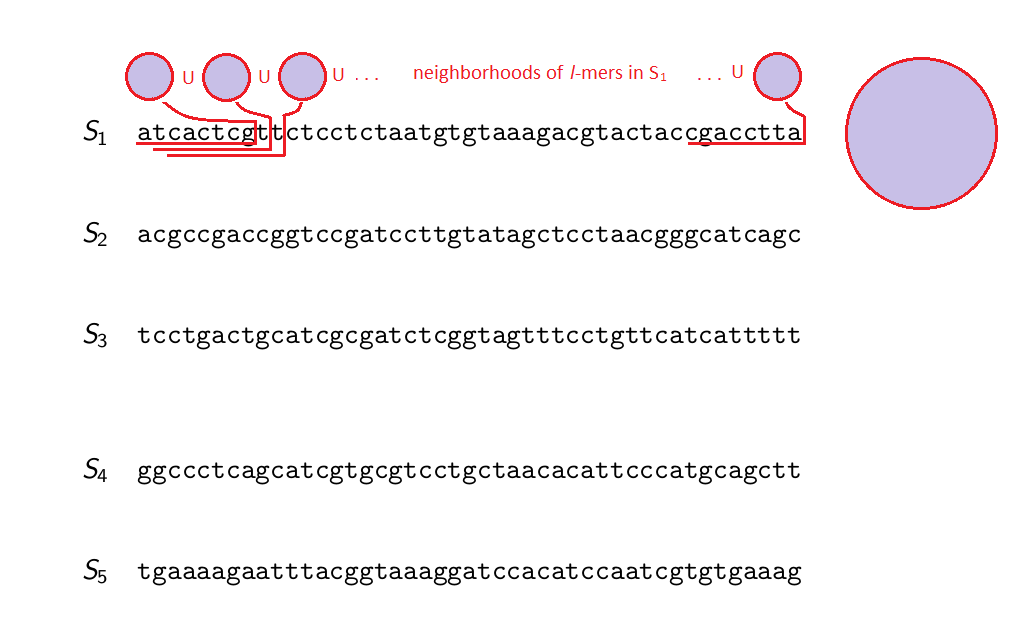
\includegraphics[width=\textwidth]{img/demo3}}
	\only<5>{\centering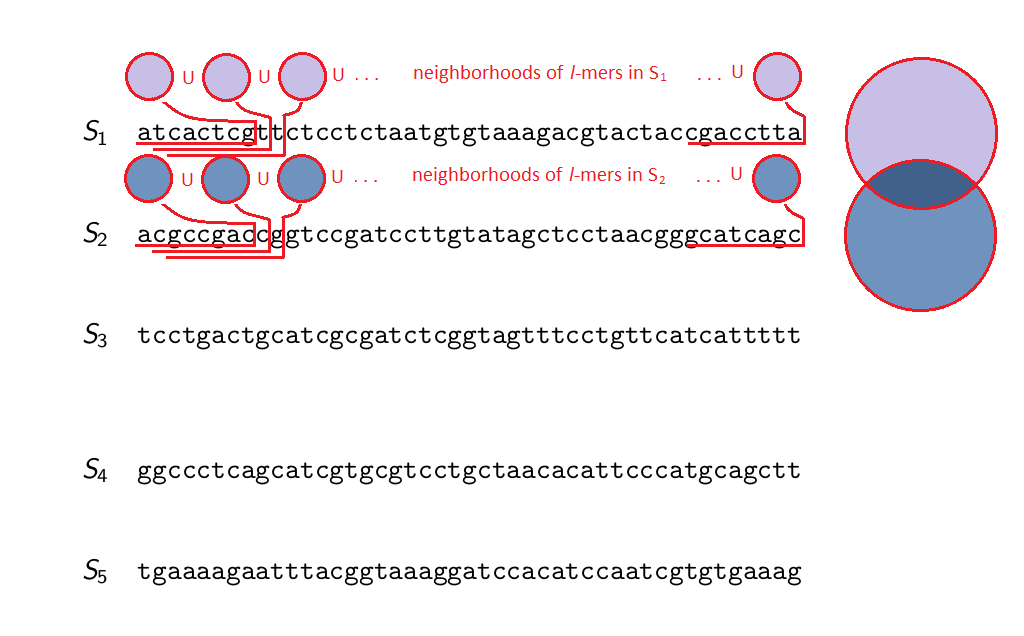
\includegraphics[width=\textwidth]{img/demo4}}
	\only<6>{\centering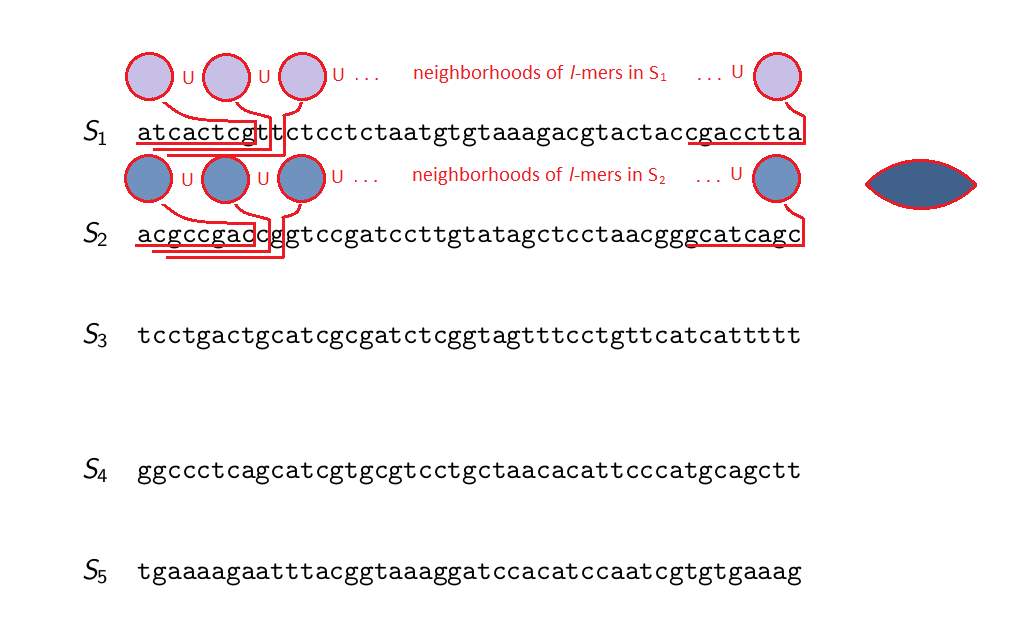
\includegraphics[width=\textwidth]{img/demo5}}
	\only<7>{\centering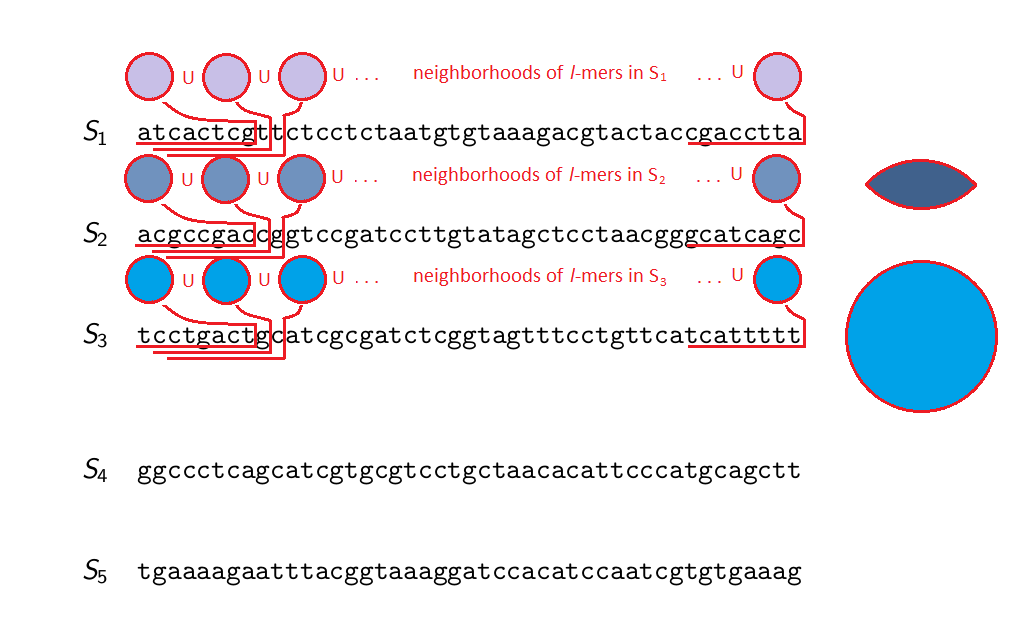
\includegraphics[width=\textwidth]{img/demo6}}
	\only<8>{\centering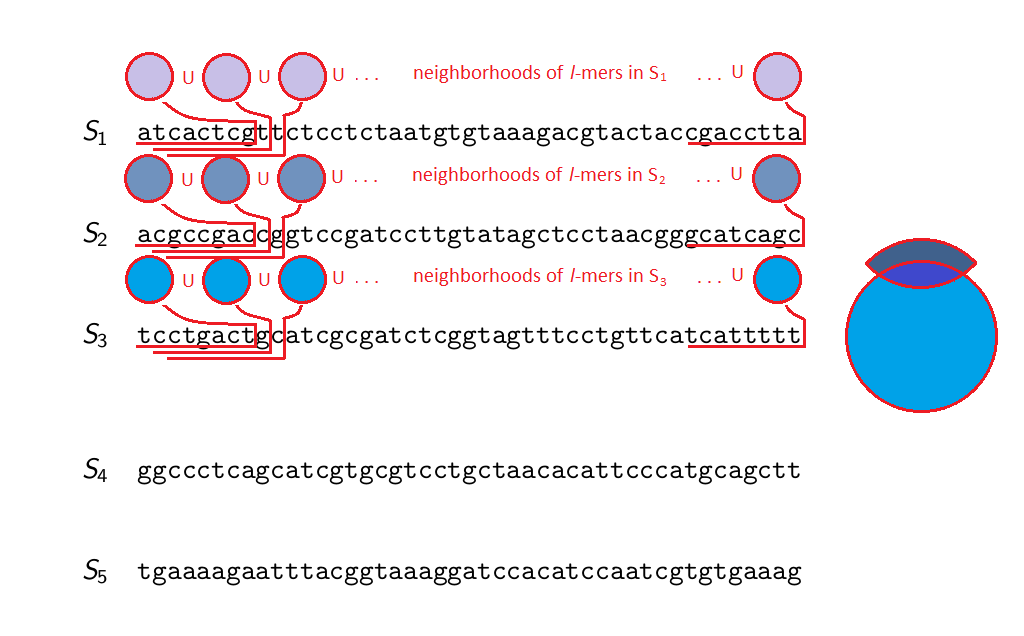
\includegraphics[width=\textwidth]{img/demo7}}
	\only<9>{\centering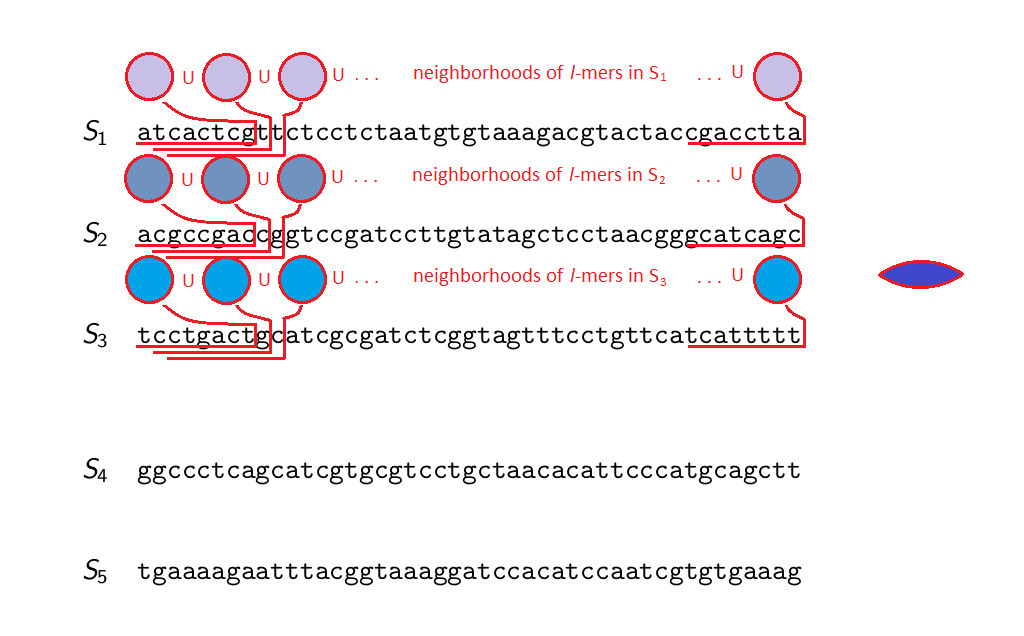
\includegraphics[width=\textwidth]{img/demo8}}
	\end{frame}

\begin{frame}{EMS-GT}{Introduction}
	\begin{itemize}
		\item {\color{red}exact motif search} (EMS) algorithm\\\vspace*{6pt}
		\begin{itemize}\normalsize
			\item {\em exact} - performs an {exhaustive search} for possible motifs\\\vspace*{6pt}
			\ \ \ \ \ \ \ - as opposed to {\em heuristic} methods
			\end{itemize}
		\ \\\ \\
		\item uses a {\color{red}generate-and-test} (GT) search approach\\\vspace*{6pt}
		\begin{itemize}\normalsize
			\item {\em generate} - narrows the search to a {set of candidate motifs}\\\vspace*{6pt}
			\item {\em test} - {checks each candidate} to see if it is a motif
			\end{itemize}
		\end{itemize}
	\end{frame}

\begin{frame}{EMS-GT}{Representing sets}
	\only<1>{
	\begin{itemize}
		\item EMS-GT must operate on sets of $l$-mers.\\\ \\
		\item There are $4^l$ possible $l$-mers that can be formed with \{\texttt{a},\texttt{c},\texttt{g},\texttt{t}\}\\\ \\
		\item Thus, {\color{red}to represent a set of $l$-mers, EMS-GT uses $4^l$ bits},
			\begin{itemize}
				\item set to 1 if the corresponding $l$-mer is a member of the set,
				\item set to 0 otherwise.
				\end{itemize}\ \\\ \\
		\item For efficiency, EMS-GT stores the $4^l$ bits as {\color{red}$\frac{4^l}{32}$ 32-bit integers}.
		\end{itemize}
		}
	\only<2->{
	\begin{itemize}
			\item $N$(\ \texttt{acgt}, 1\ )\ \ \ \ $l$=4;\ \ $4^l$ = 256, $\frac{4^l}{32}$ = 8
		\end{itemize}\ \\
	}
	\only<2>{ \centering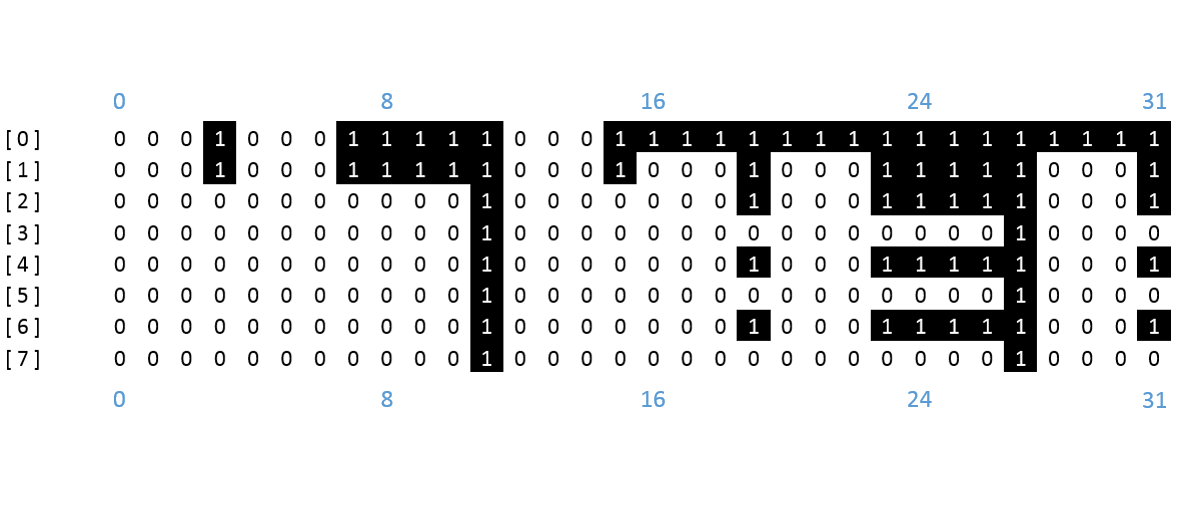
\includegraphics[width=\textwidth]{img/acgt1.png}\\ }
	\only<3>{ \centering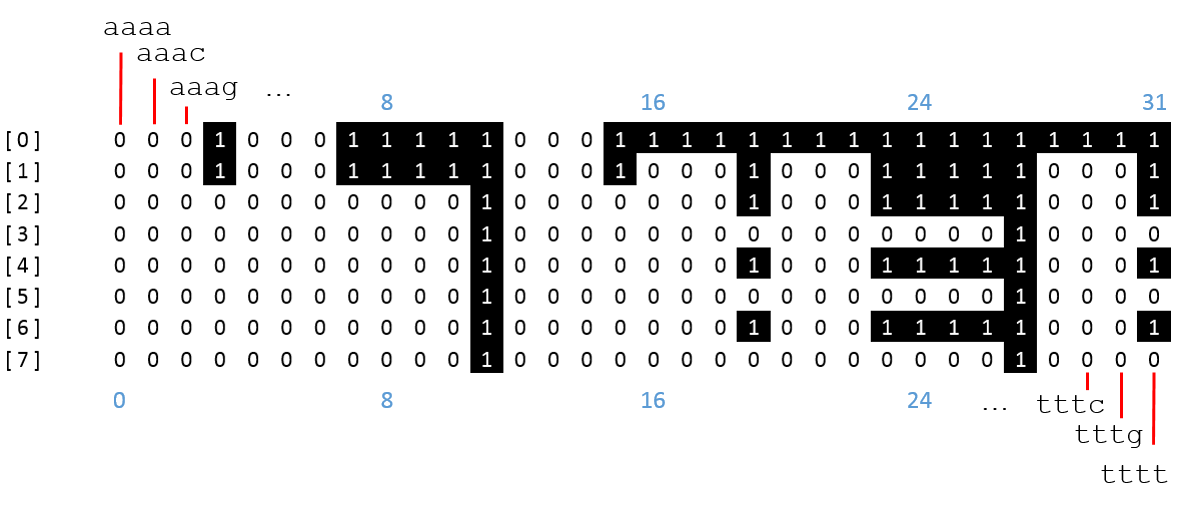
\includegraphics[width=\textwidth]{img/acgt2.png}\\ }
	\only<4>{ \centering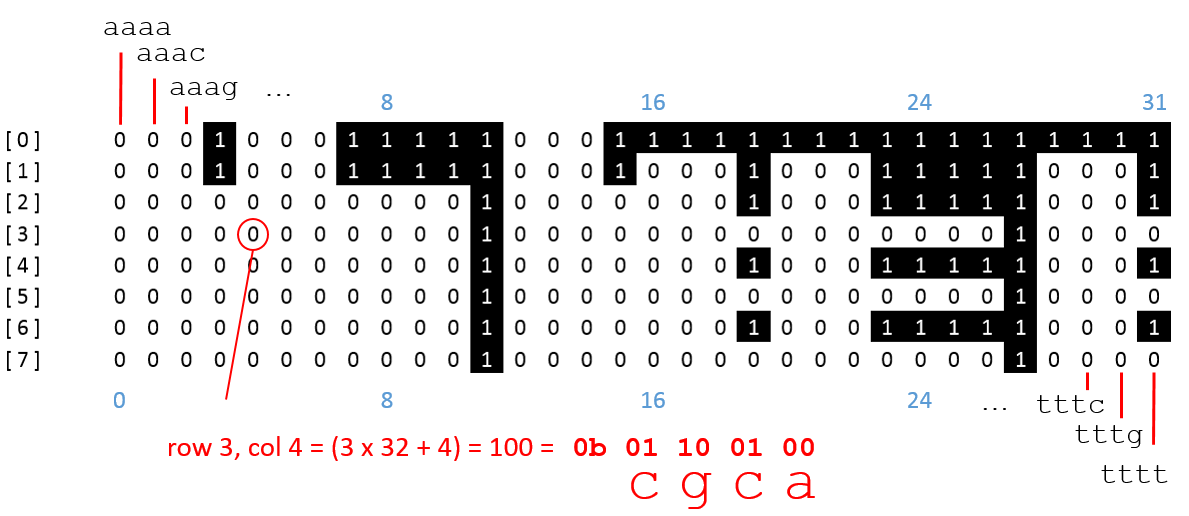
\includegraphics[width=\textwidth]{img/acgt3.png}\\ }
	\end{frame}

\begin{frame}{EMS-GT}{Generating $d$-neighborhoods}
	{\titlecolor Q: {\em How can we generate the neighborhood of an $l$-mer $x$?}}\\
	\begin{itemize}
		\only<1>{
			\item generate each $d$-neighbor, find its bit flag, and set to 1?\\\ \\
			{\centering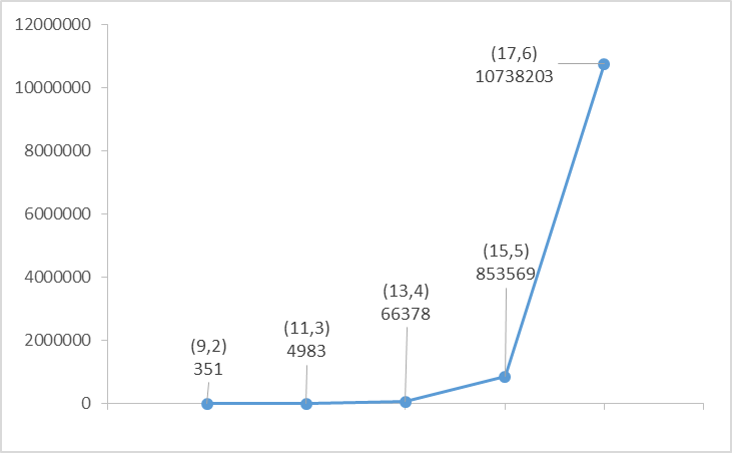
\includegraphics[width=0.8\textwidth]{img/nbrhd_growth}\\}
			}
		\only<2>{
			\item generate the neighborhood in blocks, using {\color{red} ($k$+2) patterns}\small \\
			\begin{itemize}
				\item use the {\color{red} last $k$ characters of $x$} to determine the patterns\\
				\item use the {\color{red} first $l-k$ characters of $x$} to assign patterns to blocks\\\ \\
				\end{itemize}

			\begin{columns}
			\scriptsize\centering
			\begin{column}{.135\textwidth}\centering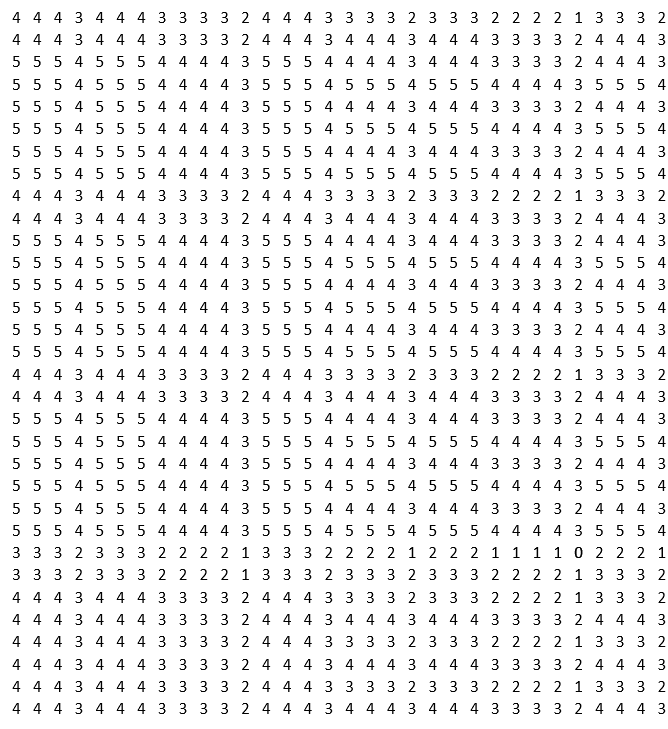
\includegraphics[width=0.98\textwidth]{img/-1}\\Pattern -1\end{column}
			\begin{column}{.135\textwidth}\centering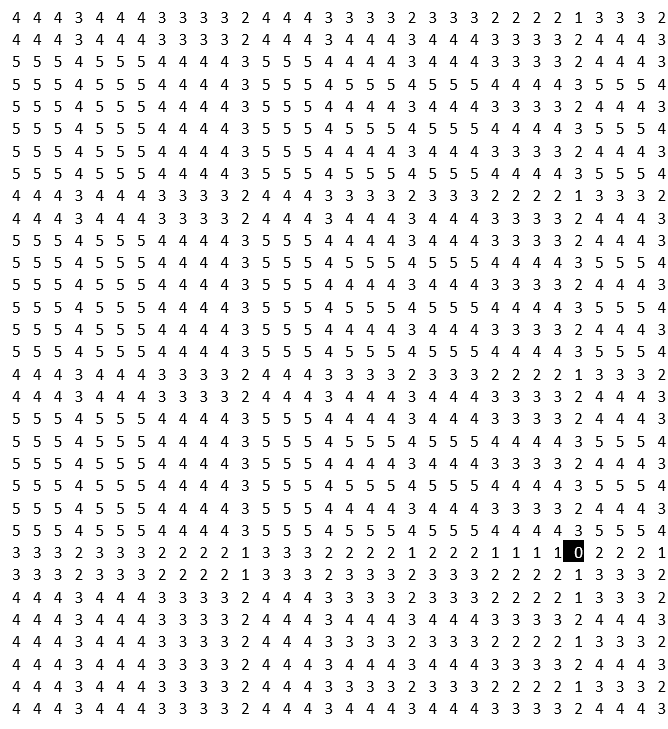
\includegraphics[width=0.98\textwidth]{img/0}\\Pattern 0 \end{column} 
			\begin{column}{.135\textwidth}\centering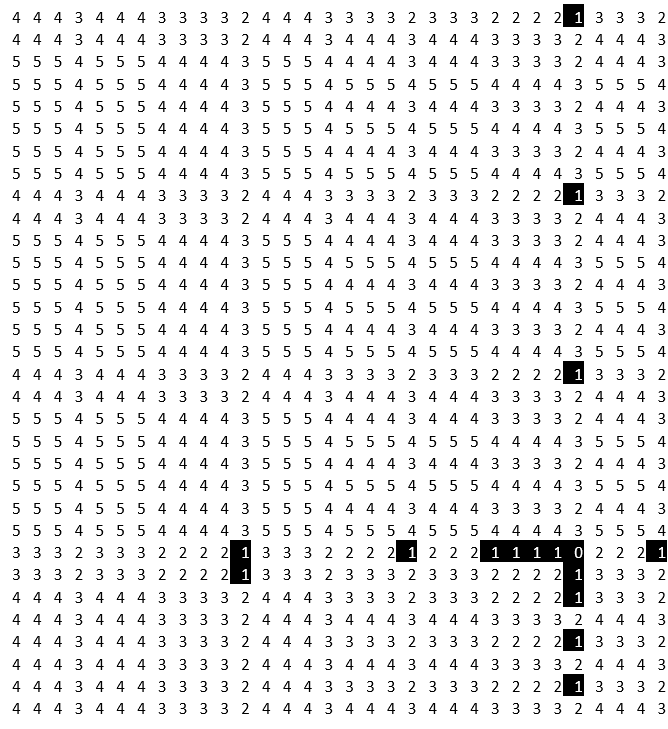
\includegraphics[width=0.98\textwidth]{img/1}\\Pattern 1 \end{column}
			\begin{column}{.135\textwidth}\centering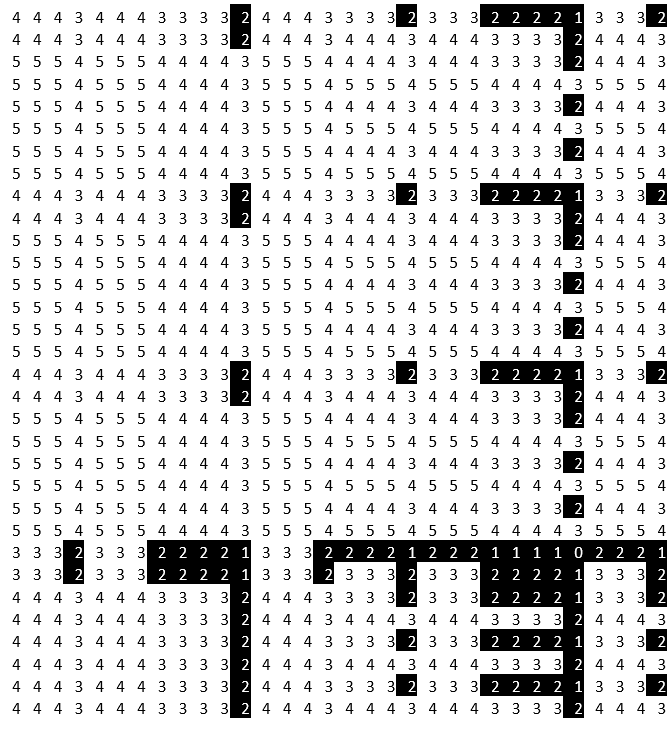
\includegraphics[width=0.98\textwidth]{img/2}\\Pattern 2 \end{column}
			\begin{column}{.135\textwidth}\centering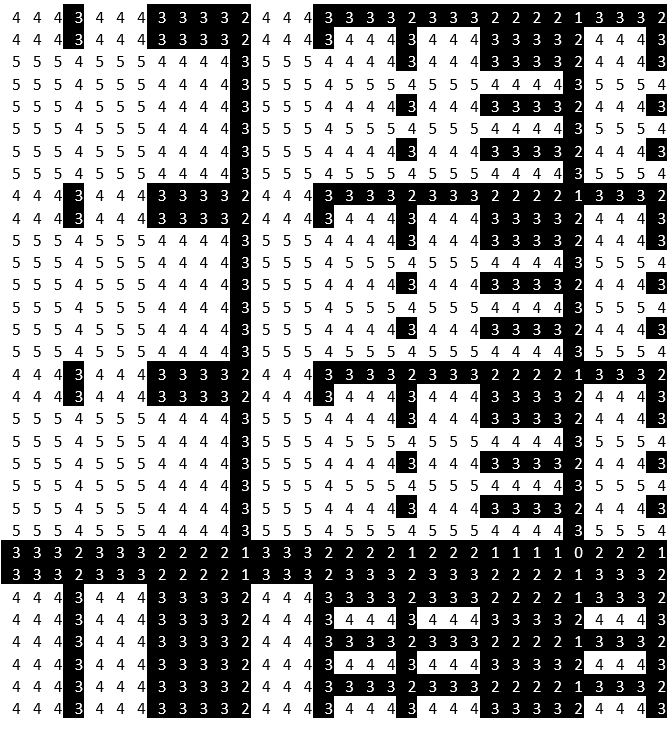
\includegraphics[width=0.98\textwidth]{img/3}\\Pattern 3 \end{column}
			\begin{column}{.135\textwidth}\centering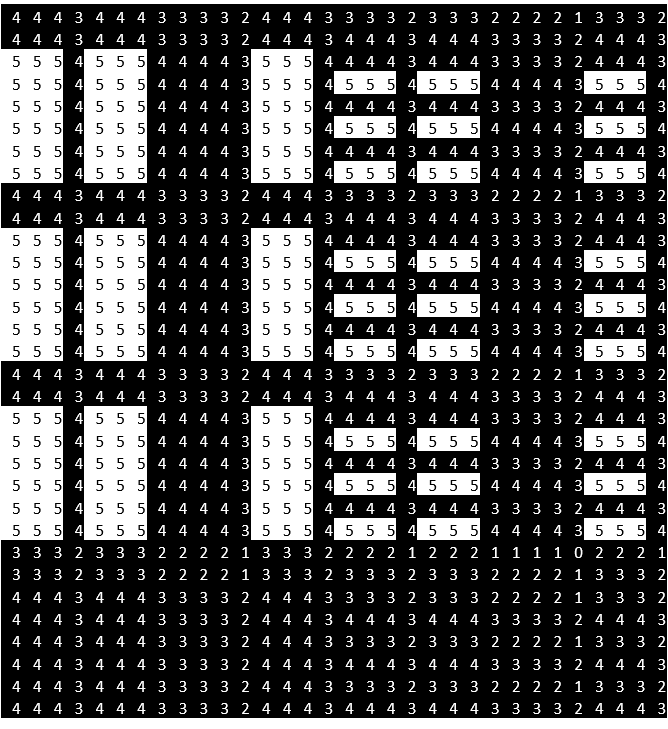
\includegraphics[width=0.98\textwidth]{img/4}\\Pattern 4 \end{column}
			\begin{column}{.135\textwidth}\centering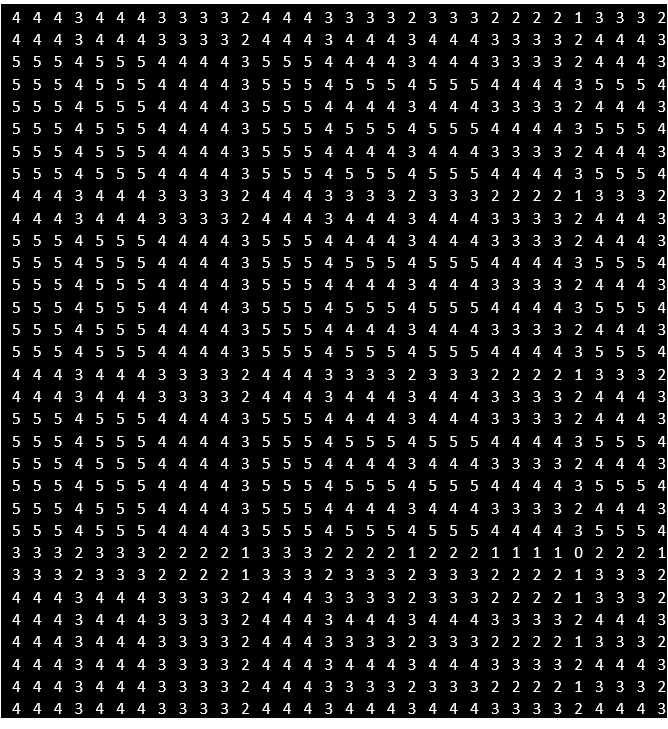
\includegraphics[width=0.98\textwidth]{img/5}\\Pattern 5 \end{column}
			\end{columns}

			}
		\end{itemize}
	\end{frame}


\begin{frame}{EMS-GT}{Building sets in blocks}
	
	\end{frame}

\begin{frame}{EMS-GT}{Results}

	\end{frame}

\end{document}